\begin{center}
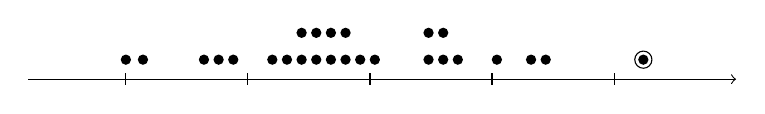
\begin{tikzpicture}[scale=0.62]
\draw[->] (0,0)--(14.5,0);
\foreach \x in {2,4.5,7,9.5,12} \draw (\x,0.12)--(\x,-0.12);
\foreach \x in {2.0,2.35,3.6,3.9,4.2,5.0,5.3,5.6,5.9,6.2,6.5,6.8,7.1,8.2,8.5,8.8,9.6,10.3,10.6} \fill (\x,0.4) circle (3pt);
\foreach \x in {5.6,5.9,6.2,6.5,8.2,8.5} \fill (\x,0.95) circle (3pt);
\draw (12.6,0.4) circle (5pt);
\fill (12.6,0.4) circle (3pt);
\end{tikzpicture}
\end{center}

中显示了唯一的一个大观测值(带圈的点).

在二维情形中, 情况较为复杂. \hyperref[fig:4.10]{图 4.10} 显示了有两个异常观测值的情况.

\begin{mvfigure}
\centering
\begin{tikzpicture}[scale=0.72]
\draw[->] (0,0)--(8.8,0) node[right,font=\small]{$x_{1}$};
\draw[->] (0,0)--(0,9.6) node[above,font=\small]{$x_{2}$};
% x2 的垂直边缘点图
\foreach \y in {0.5,0.8,1.1,1.35,1.5,1.65,1.8,2.0,2.15,2.3,2.45,2.6,2.75,2.9,3.05,3.2,3.35,3.5,3.65,3.8,3.95,4.1,4.3,4.5,4.7,4.9,5.1,5.3,5.5,5.7,5.9,6.1,6.3,6.5} \fill (1.0,\y) circle (2.2pt);
% 散布点云
\foreach \p in {(2.6,1.4),(3.0,1.6),(3.3,1.3),(3.6,2.0),(3.9,2.4),(4.2,2.2),(4.4,2.7),(4.6,3.0),(4.8,3.3),(5.0,2.9),(5.2,3.5),(5.4,3.8),(5.6,3.6),(5.8,4.1),(6.0,4.3),(6.2,4.0),(6.4,4.5),(6.6,4.2),(6.8,4.7),(7.0,5.0),(7.2,4.6),(7.4,5.2),(7.6,5.4),(6.3,5.0),(6.5,5.4),(5.9,4.8),(5.6,4.6),(5.2,4.4),(4.8,3.9),(4.4,3.4)} \fill \p circle (2.2pt);
% 带圈的离群值
\draw (1.0,8.4) circle (5pt); \fill (1.0,8.4) circle (2.2pt);
\draw (6.2,7.5) circle (5pt); \fill (6.2,7.5) circle (2.2pt);
\draw (6.6,2.0) circle (5pt); \fill (6.6,2.0) circle (2.2pt);
% x1 的底部边缘点图
\foreach \x in {0.6,0.9,1.2,1.5,1.8,2.1,2.4,2.7,3.0,3.3,3.6,3.9,4.2,4.5,4.8,5.1,5.4,5.7,6.0,6.3,7.0,7.3} \fill (\x,-0.8) circle (2.2pt);
\draw (6.6,-0.8) circle (5pt); \fill (6.6,-0.8) circle (2.2pt);
\end{tikzpicture}
\phantomsection\label{fig:4.10}\mvcap{图 4.10\quad 两个离群值: 一个单变量和一个双变量}
\end{mvfigure}

该图右上角带圈的数据点远离图中的图形, 并且它的第二个坐标较其余的 $x_{2}$ 的测量值大, 正如垂直点图所显示的. 也用圆圈圈起的第二个离群值远离其余点的椭圆形状, 但分别来看, 它的每一个分量都有一个正常的值. 这个离群值不可能靠观察边缘点图搜寻出来.

在高维中, 可能有的离群值不能从单变量散布图或者甚至二维散布图中搜寻出来. 在这里, $(\mathbf{x}_{j}-\bar{\mathbf{x}})'\mathbf{S}^{-1}(\mathbf{x}_{j}-\bar{\mathbf{x}})$ 的大值表明有异常观测值, 即使它不能直观地看到.

\mvsub{搜寻离群值的步骤}

\begin{enumerate}[label=\arabic*.,leftmargin=2em,itemsep=2pt]
\item 对于每个变量作一个点图.
\item 对于每对变量作一个散布图.
\item 对于 $j=1,2,\cdots,n$ 和每列 $k=1,2,\cdots,p$, 计算标准化值 $z_{jk}=(x_{jk}-\bar{x}_{k})/\sqrt{s_{kk}}$, 检查这些标准化值中的大值和小值.
\item 计算广义平方距离 $(\mathbf{x}_{j}-\bar{\mathbf{x}})'\mathbf{S}^{-1}(\mathbf{x}_{j}-\bar{\mathbf{x}})$, 对异常大的值检查这些距离. 在卡方图中, 这些点应当是离原点最远的点.
\end{enumerate}

步骤 3 中, “大”应当理解为与样本容量和变量个数相比较而言. 有 $n\times p$ 个标准化值. 当 $n=100$ 且 $p=5$ 时, 有 500 个值. 即使数据来自一个恰好正态的多元分布, 可预期这些值中的 1 或 2 个大于 3 或小于 $-3$. 对于一个中等的样本容量, 作为一个指标, 3.5 可以认为是大的.

在步骤 4 中, “大”是由自由度为 $p$ 的卡方分布的一个恰当的百分位数来度量的. 如果样
